\documentclass[11pt,a4paper]{article}
\usepackage[slovak]{babel}
\usepackage[utf8]{inputenc}
\usepackage[T1]{fontenc}
\usepackage{graphicx}
\usepackage{amsmath}
\usepackage{amssymb}
\usepackage{lmodern}
\usepackage{indentfirst}
\usepackage{titling}

\renewcommand{\labelenumi}{{\normalfont (\alph{enumi})}}
\renewcommand{\labelenumii}{{\normalfont \roman{enumii}.}}
\newcommand{\nN}{\ensuremath{\mathbb N}}
\newcommand{\nA}{\ensuremath{\mathcal A}}
%%%%%%%%%%%%%%%%%%%%%%%%%%%%%%%%%%%%%%%%%%%%%%%%%%%%%%%%%%%%%%%%%%%%%%%%%%%%%%%%
%%%                                                                          %%%
%%%%%%%%%%%%%%%%%%%%%%%%%%%%%%%%%%%%%%%%%%%%%%%%%%%%%%%%%%%%%%%%%%%%%%%%%%%%%%%%
\begin{document}
    %%%%%%%%%%%%%%%%%%%%%%%%%%%%%%%%%%%%%%%%%%%%%%%%%%%%%%%%%%%%%%%%%%%%%%%%%%%%%%%%
    %%%                                                                          %%%
    %%%%%%%%%%%%%%%%%%%%%%%%%%%%%%%%%%%%%%%%%%%%%%%%%%%%%%%%%%%%%%%%%%%%%%%%%%%%%%%%
    \title{Databázy (2) - Dátový model (2)}
    \author{Matej Kormuth, 2. ročník}
    %\date{}
    \date{\today}

    \begin{titlingpage}
        \renewcommand\maketitlehooka{\null\mbox{}\vfill}
        \renewcommand\maketitlehookd{\vfill\null}
        \maketitle
    \end{titlingpage}

    %%%%%%%%%%%%%%%%%%%%%%%%%%%%%%%%%%%%%%%%%%%%%%%%%%%%%%%%%%%%%%%%%%%%%%%%%%%%%%%%
    %%%                                                                          %%%
    %%%%%%%%%%%%%%%%%%%%%%%%%%%%%%%%%%%%%%%%%%%%%%%%%%%%%%%%%%%%%%%%%%%%%%%%%%%%%%%%
    \section*{ER model}

    Nalsedujúci diagram dokumentuje plánované entity a vzťahy medzi nimi.

    \begin{figure}[h]
        \centering
        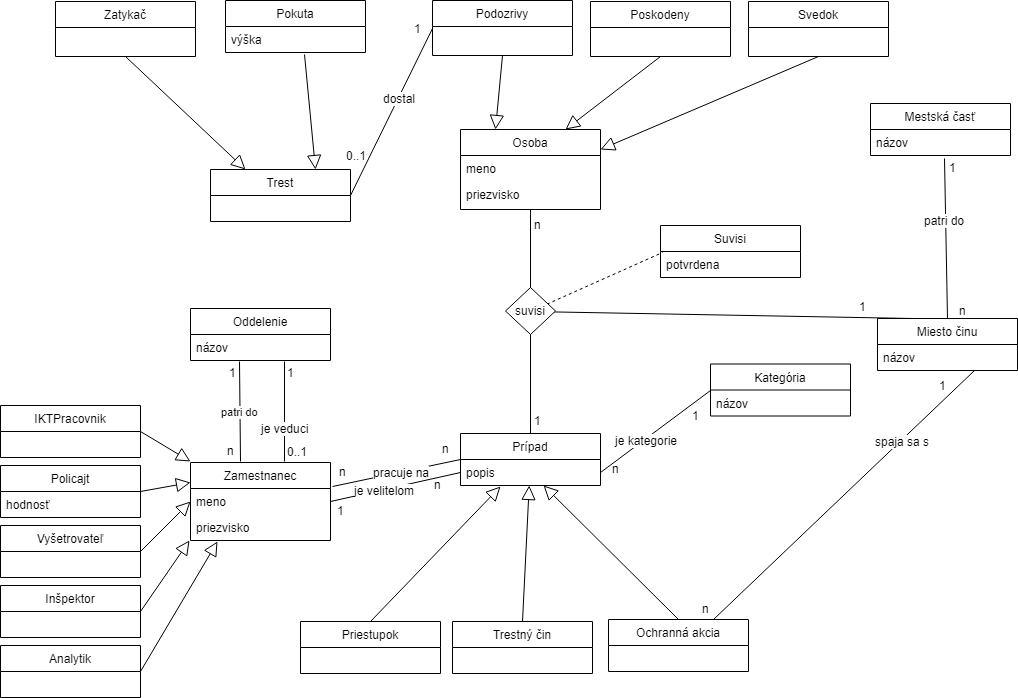
\includegraphics[width=\textwidth]{model2.png}
        \caption{Entitno-relačný diagram}
        \label{fig:my_label}
    \end{figure}

    Triedy IKTPracovník, Policajt, Vyšetrovateľ, Inšpektor a Analytik sú všetky potomkami Zamestnanca. Ak je zamestnanec Policajt, má aj svoju hodnosť.
    \\
    \\
    Každý zamestnanec je priradený do nejakého oddelenia a každé oddelenie má jedného vedúceho.
    \\
    \\
    Každý zamestnanec môže pracovať na veľa prípadoch, na jednom prípade môže pracovať viacero zamestnancov. Zároveň má každý prípad jedného veliteľa.
    \\
    \\
    Každý prípad je buď priestupok, trestný čin alebo orchranná akcia. Každý prípad má aj nejakú kategóriu. Každá kategória má svoj názov.
    \\
    \\
    Ochranné akcie nesúvisia so žiadnymi osobami, ale majú miesto činu.
    \\
    \\
    V rámci jedného prípadu existuje veľa súvislostí. Jedna súvislosť súvisí práve s jedným prípadom, jednou osobou, jedným miestom činu. Zároveň má tento vzťah aj atribút, či je potvrdený.
    \\
    \\
    To s akými miestami činu prípad súvisí sa dá zistiť zjednotením všetkých miest činu tohoto vzťahu.
    \\
    \\
    Každé miesto činu patrí nejakej mestskej časti. Každé miesto činu má svoj názov / adresu. Každá mestská čast má svoj názov.
    \\
    \\
    Každý podozrivý môže dostať trest (ak je jeho súvislosť potvrdená).
    \\
    \\
    Každý trest je buď zatykač alebo pokuta. Ak je to pokuta, tak má výšku.
    \\
    \\
    %%%%%%%%%%%%%%%%%%%%%%%%%%%%%%%%%%%%%%%%%%%%%%%%%%%%%%%%%%%%%%%%%%%%%%%%%%%%%%%%
    %%%                                                                          %%%
    %%%%%%%%%%%%%%%%%%%%%%%%%%%%%%%%%%%%%%%%%%%%%%%%%%%%%%%%%%%%%%%%%%%%%%%%%%%%%%%%
\end{document}
%%%%%%%%%%%%%%%%%%%%%%%%%%%%%%%%%%%%%%%%%%%%%%%%%%%%%%%%%%%%%%%%%%%%%%%%%%%%%%%%
%%%                                                                          %%%
%%%%%%%%%%%%%%%%%%%%%%%%%%%%%%%%%%%%%%%%%%%%%%%%%%%%%%%%%%%%%%%%%%%%%%%%%%%%%%%%